%Document Props
%FONT SIZE
%DOC CLASS
\documentclass[12pt, a4paper]{report}

%Packages
\usepackage{fullpage} %1-inch margins
\usepackage{setspace} %double space
\usepackage[backend=bibtex8]{biblatex}
\addbibresource{ref.bib}
%Change Chapter format in report class
\usepackage{titlesec} 
\titleformat{\chapter}[block]
  {\normalfont\huge\bfseries}{\thechapter.}{1em}{\Huge}
\titlespacing*{\chapter}{0pt}{-19pt}{0pt}

%Graphics package and relative path
\usepackage{graphicx}
\graphicspath{{images/}}

% For other font sizes
% !incompatible with fullpage
%\usepackage{extsizes}

\onehalfspacing
% ----------------------------------------------------------------------------------------------
\begin{document}

% Outer Cover Page
\pagestyle{empty}
\begin{titlepage}
\vspace*{0.2cm}
\begin{center} \textbf{A REPORT\\ON} \end{center}
\begin{center} \textbf{{\Large AUTOMATIC LAND COVER CLASSIFICATION OF MULTI-TEMPORAL SATELLITE IMAGES}} \end{center}
\begin{center} \textbf{BY} \end{center}
\begin{center} 
{\Large 
	\begin{tabular}{c c}
	Guntaas Singh & 2018A7PS0269P\\
	Nisarg Vora & 2018A7PS0254P
	\end{tabular}
}
\end{center}
\begin{center} \textbf{AT} \end{center}
\begin{center} 
\includegraphics{iirs.png} \end{center}
\begin{center} {\Large Indian Institute of Remote Sensing, Dehradun} \end{center}
\begin{center} A Practice School - I station of \end{center}
\begin{center} {
\includegraphics{bits.png}} \end{center}
\begin{center} {\Large Birla Institute of Technology and Science, Pilani} \end{center}
\begin{center} June, 2020 \end{center}
\end{titlepage}
\pagebreak

% Inner Cover Page
\begin{titlepage}
\vspace*{0.3cm}
\begin{center} \textbf{A REPORT\\ON} \end{center}
\begin{center} \textbf{{\Large AUTOMATIC LAND COVER CLASSIFICATION OF MULTI-TEMPORAL SATELLITE IMAGES}} \end{center}
\begin{center} \textbf{BY} \end{center}
\begin{center}
	\begin{tabular}{c c c}
		\textbf{ID Number} & \textbf{Name} & \textbf{Branch} \\
		2018A7PS0269P & Guntaas Singh & B.E. (Hons.) Computer Science \\
		2018A7PS0254P & Nisarg Vora  & B.E. (Hons.) Computer Science \\
	\end{tabular} 
\end{center}
\begin{onehalfspace}
\begin{center} \textbf{Prepared in the partial fulfillment of the} \end{center}
\begin{center} Practice School - I course \end{center}
\begin{center} \textbf{AT} \end{center}
\begin{center} 
\includegraphics{iirs.png} \end{center}
\begin{center} {\Large Indian Institute of Remote Sensing, Dehradun} \end{center}
\begin{center} A Practice School - I station of \end{center}
\begin{center} {
\includegraphics{bits.png}} \end{center}
\begin{center} {\Large Birla Institute of Technology and Science, Pilani} \end{center}
\begin{center} June, 2020 \end{center}
\end{onehalfspace}
\end{titlepage}
\pagebreak

% Acknowledgements
\setcounter{secnumdepth}{0}
\section{Acknowledgments}
\pagestyle{plain}
\pagenumbering{roman}
\setcounter{page}{3}
\paragraph{}
We would sincerely like to thank the Director of Indian Institute of Remote Sensing, Dr. Prakash Chauhan, for giving us an opportunity to work in this organization and gain a significant amount of exposure to corporate work culture, ethics, and etiquette to be followed while working in a professional environment.
\paragraph{}
We would like to extend our most sincere gratitude to our project in-charge, Dr. Hari Shanker Srivastava, Head of the Programme Planning and Evaluation Group (PPEG) at IIRS, for providing us with the opportunity to work with him on this project, and his guidance and mentorship during the same.
\paragraph{}
We wish to extend our gratitude to the faculty in charge of the PS-I program at IIRS, Dr. Rekha A., Assistant Professor at BITS Pilani - Bangalore Center, for her guidance and advice during the PS-I program, and her helpfulness and responsiveness while addressing all the concerns we raised during the same.
\paragraph{}
In addition, we would also like to thank the members of the Practice School Division, who have worked very hard for operating the PS-I programme remotely to ensure that we have a seamless learning experience.
\pagebreak

% Details and abstract
\begin{center}  
\textbf {BIRLA INSTITUTE OF SCIENCE AND TECHNOLOGY\\
PILANI (RAJASTHAN)\\
Practice School Division}
\end{center}
\begin{onehalfspace}
\textbf{Station:} Indian Institute of Remote Sensing \\
\textbf{Centre:} Dehradun\\
\textbf{Duration:} From 18th May, 2020 to 27th June, 2020 \\
\textbf{Date of start:} 18th May, 2020 \\
\textbf{Date of submission:} 4th June, 2020 \\
\textbf{Title of project:} Automatic Land Cover Classification of Multi-temporal Satellite Images
\begin{center}
\begin{tabular}{c c c}
\textbf{ID Number} & \textbf{Name} & \textbf{Branch} \\
2018A7PS0269P & Guntaas Singh & B.E. (Hons.) Computer Science \\
2018A7PS0254P & Nisarg Vora  & B.E. (Hons.) Computer Science \\
\end{tabular} 
\end{center}
\textbf{Name of guide:} Dr. Hari Shanker Srivastava \\
\textbf{Designation:} Scientist/Engineer - SG. Group Head, Programme Planning and Evaluation Group (PPEG). \\
\textbf{Name of PS faculty:} Dr. Rekha A. 

	\section{Abstract}
	\paragraph{}
	Blah
\end{onehalfspace}
\newpage

%Response sheet
\begin{center}  
\textbf {BIRLA INSTITUTE OF SCIENCE AND TECHNOLOGY\\
PILANI (RAJASTHAN)\\
Practice School Division\\
Response Option Sheet}
\end{center}
\begin{onehalfspace}
\textbf{Station:} Indian Institute of Remote Sensing \\
\textbf{Centre:} Dehradun
\begin{center}
\begin{tabular}{c c c}
\textbf{ID Number} & \textbf{Name} & \textbf{Branch} \\
2018A7PS0269P & Guntaas Singh & B.E. (Hons.) Computer Science \\
2018A7PS0254P & Nisarg Vora  & B.E. (Hons.) Computer Science \\
\end{tabular} 
\end{center}
\textbf{Title of project:} Automatic Land Cover Classification of Multi-temporal Satellite Images\\
\begin{center}
\begin{tabular}{|p{1cm}|p{10cm}|p{3cm}|}
\hline
\textbf{Code No.} & \textbf{Response Option} & \textbf{Course No.(s) and Name} \\
\hline
1 & A new course can be designed out of this project. & ~\\
\hline
2 & The project can help modification of the course content of some of the existing Courses & ~\\
\hline
3 & The project can be used directly in some of the existing Compulsory Discipline Courses (CDC)/ Discipline Courses Other than Compulsory (DCOC)/ Emerging Area (EA), etc. Courses & ~\\
\hline
4 & The project can be used in preparatory courses like Analysis and Application Oriented Courses (AAOC)/ Engineering Science (ES)/ Technical Art (TA) and Core Courses. & ~\\
\hline
5 & This project cannot come under any of the above mentioned options as it relates to the professional work of the host organization. &~ \\
\hline
\end{tabular} 
\end{center}
\end{onehalfspace}
\vspace*{0.5cm}
\textbf{Signature}\\
\textbf{Date: }
\newpage

% Table of Contents
\tableofcontents
\newpage

% INTRODUCTION
\setcounter{page}{1}
\setcounter{secnumdepth}{1}
\chapter{Introduction}
\pagenumbering{arabic}
\section{About IIRS}
\paragraph{}
Formerly known as Indian Photo-interpretation Institute (IPI), the Institute was founded on 21st April 1966 under the aegis of Survey of India (SOI). It was established with the collaboration of the Government of The Netherlands on the pattern of Faculty of Geo-Information Science and Earth Observation (ITC) of the University of Twente, The Netherlands. The original idea of setting the Institute came from India's first Prime Minister Pandit Jawahar Lal Nehru during his visit to The Netherlands in 1957. Since its establishment in 1966, IIRS is a key player for training and capacity building in geospatial technology and its applications through training, education and research in Southeast Asia. The training, education and capacity building programmes of the Institute are designed to meet the requirements of Professionals at working levels, fresh graduates, researchers, academia, and decision makers. IIRS is also one of the most sought after Institute for conducting specially designed courses for the officers from Central and State Government Ministries and stakeholder departments for the effective utilization of Earth Observation (EO) data. Keeping pace with the technological advances, the Institute has enhanced its capability with time, to fulfill the increased responsibility and demand from Indian and international community. Today, it has programmes for all levels of users, i.e. mid-career professionals, researchers, academia, fresh graduates and policy makers. The sustained efforts by its dedicated faculty and the management have made the institute remain in the forefront throughout its journey of about four and a half decades from a photo-interpretation institute to an institute of an international stature in the field of remote sensing and geo-information science.\cite{iirs.about.history}\cite{iirs.about.instiprof}
\section{Remote Sensing}
\paragraph{}
Remote sensing is the acquisition of information about an object or phenomenon without making physical contact with the object and thus in contrast to on-site observation, especially the Earth. Remote sensing is used in numerous fields, including geography, land surveying and most Earth science disciplines (for example, hydrology, ecology, meteorology, oceanography, glaciology, geology); it also has military, intelligence, commercial, economic, planning, and humanitarian applications.  It may be split into "active" remote sensing (when a signal is emitted by a satellite or aircraft to the object and its reflection detected by the sensor) and "passive" remote sensing (when the reflection of sunlight is detected by the sensor). Passive sensors gather radiation that is emitted or reflected by the object or surrounding areas. Reflected sunlight is the most common source of radiation measured by passive sensors. Examples of passive remote sensors include film photography, infrared, charge-coupled devices, and radiometers. Active collection, on the other hand, emits energy in order to scan objects and areas whereupon a sensor then detects and measures the radiation that is reflected or backscattered from the target. RADAR and LiDAR are examples of active remote sensing where the time delay between emission and return is measured, establishing the location, speed and direction of an object. \cite{remotesensingwiki}
\section{Normalized Difference Vegetation Index(NDVI)}
\paragraph{}
Satellite data has become an integral part of modern agricultural management to keep track of crop progress. Some satellite data, however, also can foretell how a crop will perform in the future, offering valuable insights to a wide range of industry players.
NDVI is probably the most important of the satellite data. By reading infrared light waves reflected from plants, NDVI can signal stresses to plant health, such as oncoming drought, as much as two weeks before problems are visible to the naked eye. Many agricultural industry participants can benefit from such advance alerts. Farmers can increase irrigation or add crop protection to forestall a pest infestation. And physical traders, processors, and food and beverage companies could seek out alternative supplies, or hedge their positions.\\cite{ndvione}
\paragraph{}
NDVI also can reveal positive indications about a crop, providing a heads-up to market participants, logistics companies, and others to prepare for a big harvest. Another type of satellite data, called evapotranspiration (ET), also sends early-warning signals about plants, based on measures of moisture evaporation and transpiration. But ET is available only on a monthly basis, much less frequent than the eight-day reports on NDVI.\\cite{ndvione}
\subsection{What is NDVI?}
\paragraph{}
Early space exploration quickly led to atmospheric and meteorological studies. NASA in 1972 launched the Earth Resources Technology Satellite, the forerunner to Landsat, the world’s longest-running satellite imagery program. This first satellite was able to distinguish between visible red and near-infrared reflectance bands, which allowed it to identify vegetation, soil, water, and other features.\\cite{ndvione}
\paragraph{}
Light from the sun is present as visible light (reds, greens, and blues) and light not visible to our eyes (infrared and ultraviolet). These can be absorbed, transmitted, or reflected by an object. In healthy plants, most of the visible light is absorbed for use in photosynthesis, and much of the near-infrared radiation (NIR) is reflected. However, if the plant is stressed, because of dehydration, for instance, it reflects less NIR and absorbs less light in the visible spectrum, specifically in the red portion, since the plant is not using photosynthesis as efficiently.\\cite{ndvione}
\subsection{Formula}
NDVI is calculated in accordance with the formula:
\begin{center} 
\includegraphics{ndviformula.png} \end{center}
where,\\
NIR - reflection in the near-infrared spectrum
RED - reflection in the red range of the spectrum
\paragraph{}
According to this formula, the density of vegetation (NDVI) at a certain point of the image is equal to the difference in the intensities of reflected light in the red and infrared range divided by the sum of these intensities.\\
This index defines values from -1.0 to 1.0, basically, representing greens, where negative values are mainly formed from clouds, water and snow, and values close to zero are primarily formed from rocks and bare soil. Very small values (0.1 or less) of the NDVI
function correspond to empty areas of rocks, sand or snow. Moderate values (from 0.2 to 0.3) represents shrubs and meadows, while large values (from 0.6 to 0.8) indicate temperate and tropical forests. Crop Monitoring successfully utilizes this scale to show farmers which parts of their fields have dense, moderate, or sparse vegetation at any given moment. Put simply, NDVI is a measure of the state of plant health based on how the plant reflects light at certain frequencies (some waves are absorbed and others are reflected).
\begin{center} 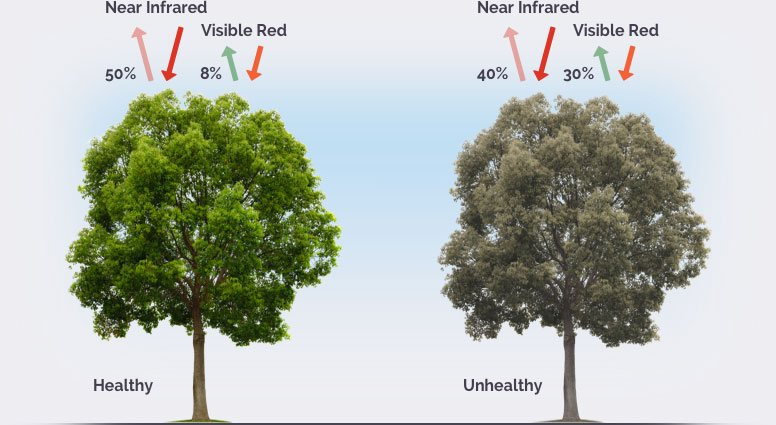
\includegraphics{ndviillustration.jpg} \end{center}
\subsection{Illustration}
\paragraph{}
Chlorophyll (a health indicator) strongly absorbs visible light, and the cellular structure of the leaves strongly reflect near-infrared light. When the plant becomes dehydrated, sick, afflicted with disease, etc., the spongy layer deteriorates, and the plant absorbs more of the near-infrared light, rather than reflecting it. Thus, observing how NIR changes compared to red light provides an accurate indication of the presence of chlorophyll, which correlates with plant health.
\begin{center} 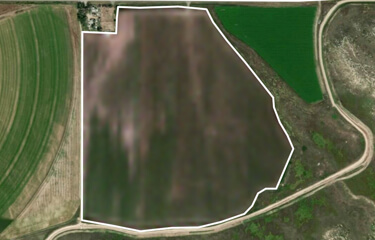
\includegraphics{ndvisampleone.jpg} \end{center}
\begin{center} \textbf{Without NDVI} \end{center}
\begin{center}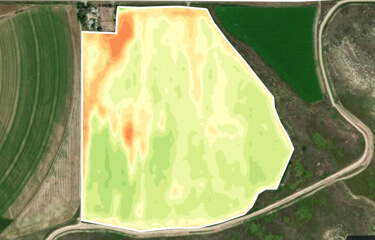
\includegraphics{ndvisampletwo.jpg} \end{center}
\begin{center} \textbf{With NDVI} \end{center}


\newpage

% ____________________________

% METHODOLOGY
\chapter{Methodology}
\section{Image Classification}

Image classification is a standard task in computer vision. In general, the image classification problem involves assigning one  label out of a given fixed set of discrete labels to the input image on the basis of its visual content. While this is a trivial task for humans, robust image classification is a big challenge for a machine. To the computer, the image is just a grid of numbers which entirely change in unreliable ways with variations in viewpoint, illumination, occlusion, etc. As a result, there is no obvious algorithm which solves this problem. However, a data driven approach of providing the machine with many examples of each class and use of machine learning techniques has shown to be useful.\cite{cs231n}
\paragraph{}
There are different ways in which these techniques can be applied for classification of satellite imagery.
\subsection{Pixel Based Approach}
In typical satellite images, pixel sizes are generally similar in size to the objects of interest. Most of the methods for image analysis using remote sensing data work on a per-pixel basis. However, with advances in remote sensing technology, the spatial resolution has become finer than the typical objects of interest, leading to an increase in within-class variability.\cite{eyesky}
\subsection{Object Based Approach}
The term "objects" represents meaningful semantic entities or scene components that are distinguishable in an image.\cite{eyesky} This approach involves the partition of the image into meaningful geographical objects that share relatively homogeneous spectral, color, etc.
\subsection{Semantic Approach}
This aims to label each scene image with a specific semantic class. Here, a scene image usually refers to a local image patch manually extracted from large scale remote sensing images that contain explicit semantic classes.\cite{eyesky}

\section{Deep Learning and Neural Networks}
Application of traditional machine learning techniques requires handcrafted features, developing which demands a considerable amount of engineering skill and domain expertise. This, however, is not true for neural networks, which automatically learn these features from data using a general-purpose learning procedure.\cite{eyesky, cs231n} Despite having been around for decades, neural networks have garnered much attention only in the last few years on account of the availability of increased computational power and large amounts of data.
\paragraph{}
A standard neural network consists of many simple, connected processors called neurons, each producing a sequence of real-valued activations. Input neurons get activated through sensors perceiving the environment, other neurons get activated through weighted connections from previously active neurons. \cite{schmidhuber2015deep} Each neuron can be seen as a single unit applying a non-linear activation function (such as sigmoid, tanh, ReLU) to a linear combination of the input activations to the neuron.\cite{cs229}
\begin{figure}[h]
\centering
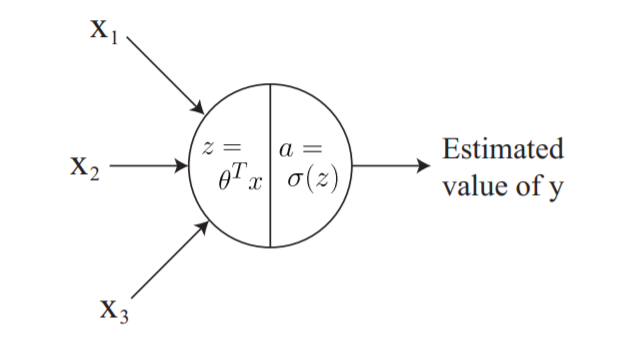
\includegraphics[width=0.5\textwidth]{nn1.png}
\caption{A single neuron.}\cite{cs229}
\end{figure}
\paragraph{}
These single neurons can be stacked so that one neuron passes its output as input into the next neuron. The resulting network of neurons can, hence, consist of several layers of neurons, each with their own learnable weights and biases. Used in conjunction with an appropriate loss function and optimization algorithm, such a network can be used to learn any complex function, if sufficient data is available for training. Forward propagation through the network yields its prediction for a given input. This prediction is compared with the actual class label, and the loss is computed. Backward Propagation is used to compute the gradients of the loss function with respect to the parameters, which are then used by the optimization algorithm to adjust the parameters and minimize the loss over a number of iterations.
\begin{figure}[h]
\centering
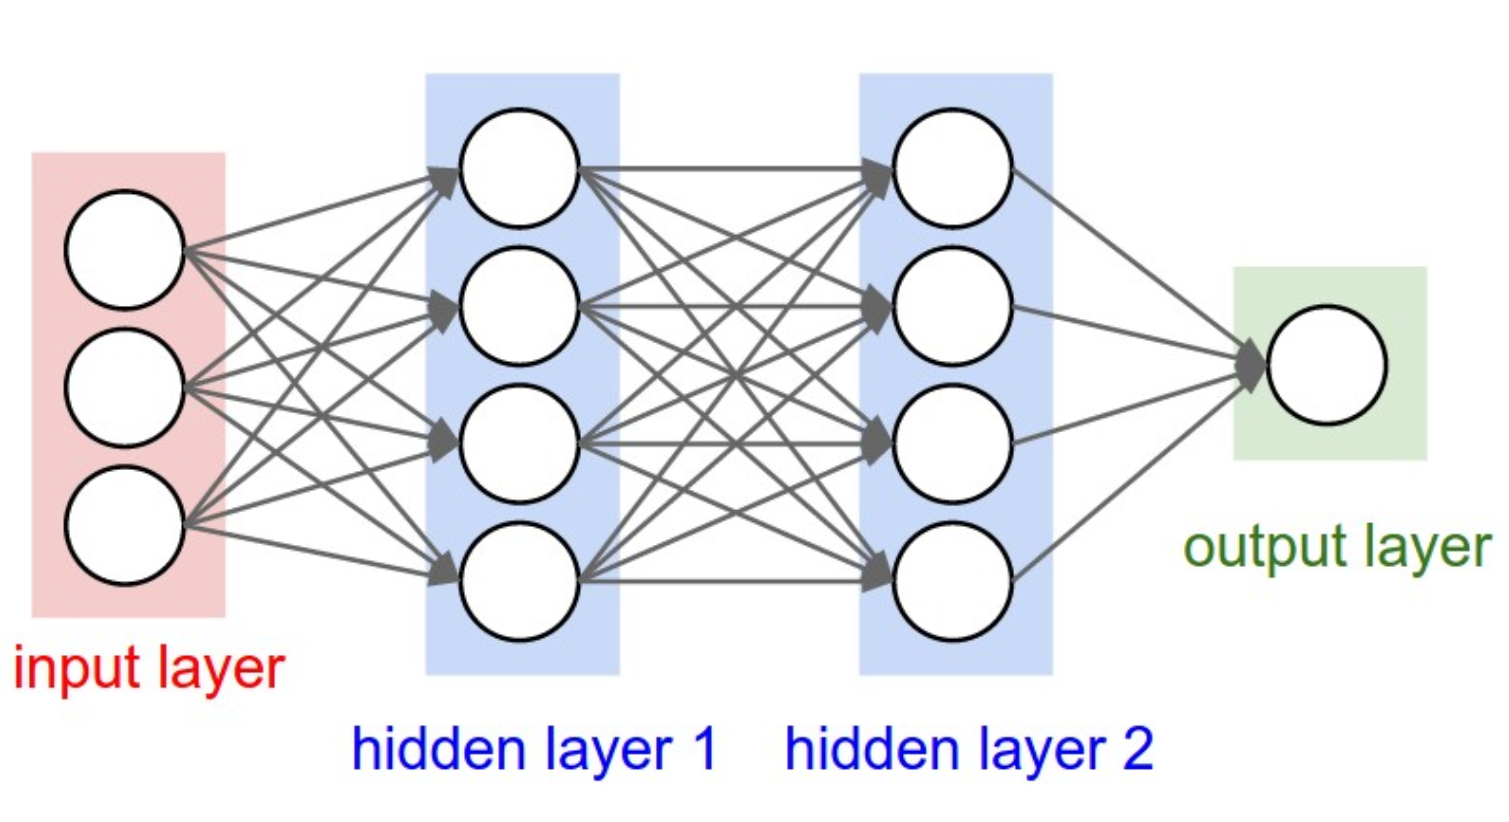
\includegraphics[width=0.7\textwidth]{nn2.png}
\caption{A two layer neural network with fully connected layers.}\cite{cs231n}
\end{figure}
\newpage

\section{Convolutional Neural Networks}
\paragraph{}
Regular neural networks do not scale well to full images. If the input to the neural network is a 200x200 RGB image, the number of weights for each neuron will be 200*200*3 = 120,000 weights. For large networks, the total number of learnable parameters become very large and lead the model to potentially overfit the training data, unless the training set is adequately large.
\paragraph{}
A convolutional neural network (CNN) is a sequence of layers. Each layers transforms an input volume (images are represented as a three dimensional matrix) of activations to another with some differentiable function which may or may not have parameters.\cite{cs231n, dlai4} These layers are of three main types:
\subsection{Convolutional Layer}
This is the core building block for convolutional networks. It is based on the convolution operation on images.
\paragraph{}
Each convolutional layer of a CNN consists of $N$ kernels or filters of a certain volume of neurons sized $f \times f \times d$, with $f$ being the spatial dimension and $d$ being the number of feature channels of the kernel, which is same as the number of channels in the image at its input ($D_{i}$). Every one of these filters is convolved with a corresponding volume of the input image, and is slid through the entire image of size $H_{i} \times W_{i} \times D_{i}$. Convolution refers to the summation of the element-wise dot product of the neurons in each filter with the corresponding values in the input, for each position in which the filter is aligned with the image. Based on this notion, a convolution with a single filter at each layer results in a two dimensional output of a certain size. \cite{cs231n, muruganandham2016semantic, dlai4}
\begin{figure}[h]
\centering
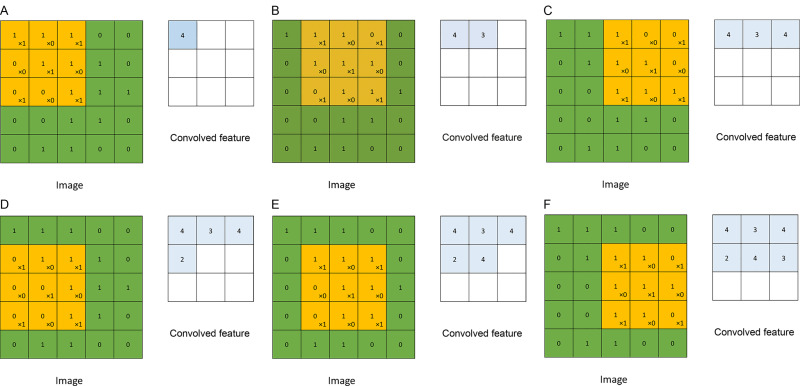
\includegraphics[width=\textwidth]{cnn1.jpg}
\caption{The convolution operation performed using a 3x3 filter on a 5x5x1 image.}\cite{fathi2018deep}
\end{figure}
\paragraph{}
The intervals with which the filter moves in each spatial dimension is decided by the \textbf{stride} $s$. In order to prevent undue shrinkage of the volume along the spatial dimension, the image can be padded with pixels along the outer edges. The width of this \textbf{padding}, in pixels, is given by another hyper-parameter, $p$.\cite{dlai4, muruganandham2016semantic} The convolution operation is repeated for each of the $N$ filters, and the resulting $N$ activation maps are stacked together across the third dimension giving an output volume of dimensions:\\
\begin{displaymath}
H_{o}=\frac{H_{i}-f+2p}{s}+1
\end{displaymath}
\begin{displaymath}
W_{o}=\frac{W_{i}-f+2p}{s}+1
\end{displaymath}
\begin{displaymath}
D_{o}=N
\end{displaymath}
\paragraph{}
In a convolutional layer, each neuron is connected to only a local region of the input volume, called the receptive field of that neuron. The extent of connectivity is limited to the filter size along the spatial dimensions, but is full along the depth axis.\cite{cs231n} It should also be noted that all activations belonging to a particular channel in the output volume correspond to a single filter applied on the input volume, and hence depend on the same shared parameters. Local connectivity and parameter sharing not only help reduce the number of learnable parameters, but also make the CNN good at capturing \textbf{translation invariance}. This makes them an ideal choice for the image classification problem.
\subsection{Pooling Layer}
It is common to periodically insert a Pooling layer in-between successive convolutional layers in a CNN. Its function is to progressively reduce the spatial size of the representation to reduce the amount of parameters and computation in the network, and hence to also control overfitting.\cite{cs231n} The most common form of pooling layer in CNN architectures employs filters of size $2 \times 2$ with a stride of 2, taking a max over 4 cells of the input image. It is worth noting that while this halves the width and height of the image, the depth remains unaffected as the max operation is applied independently to each channel of the image. This down-sampling process effectively discards 75\% of the activations.
\begin{figure}[h]
\centering
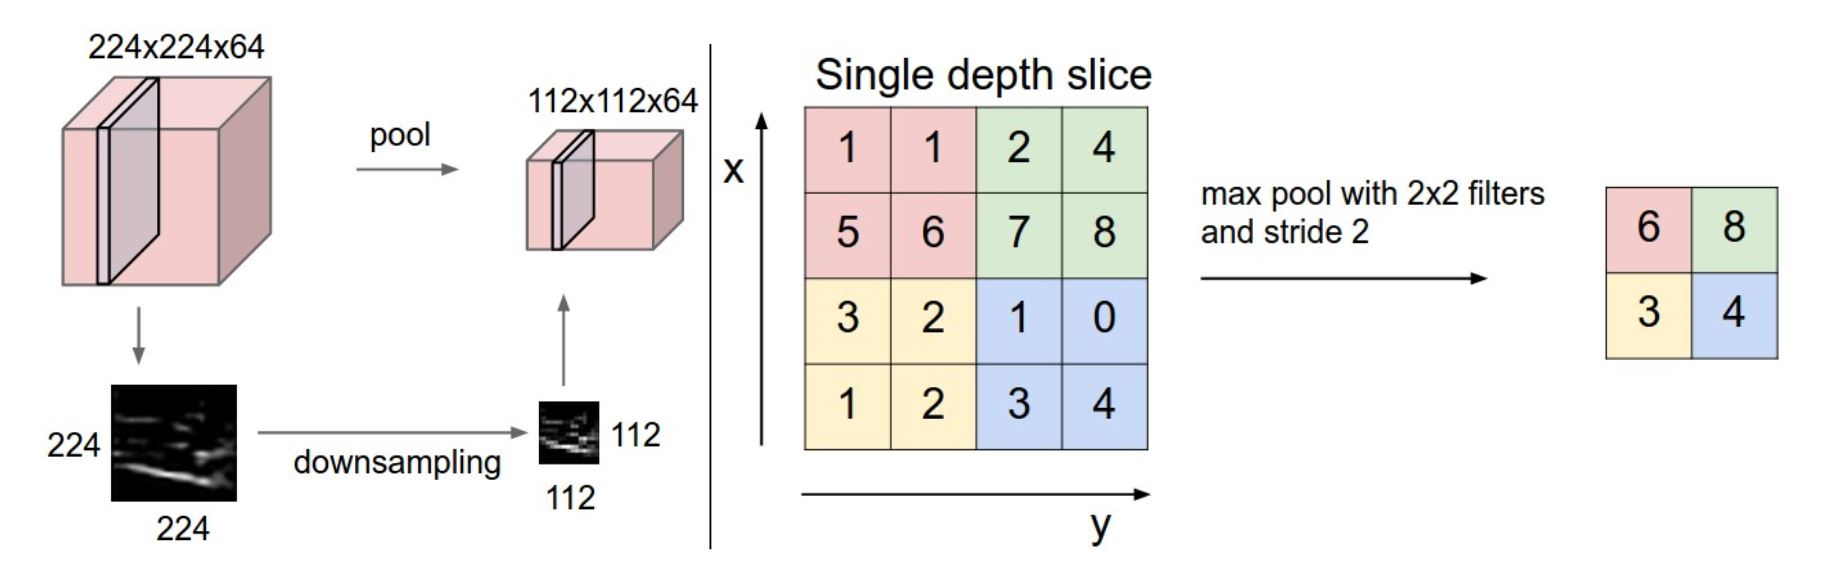
\includegraphics[width=\textwidth]{cnn2.jpg}
\caption{(1) A typical max pooling layer. (2) The max pooling operation.}\cite{cs231n}
\end{figure}
\subsection{Fully Connected Layer}
Once higher level features are detected from the preceding convolution and pooling layers, a fully connected layer is usually attached at the end of the network. This layer is fully connected to all activations in the previous layer, as in regular neural networks, allowing all the features learned by the network to be taken into account by the output layer. \paragraph{}
In practice, fully connected layers have an equivalent representation as a convolutional layer having $N$ filters with dimensions equal to those of the input image. The output of this layer will thus be a volume of dimensions $1 \times 1 \times N$. This simple change allows the same CNN to be applied on images with arbitrary spatial dimensions and classify them in a single pass of forward propagation, instead of iterating on different crops of adequate size. This is the basic intuition behind \textbf{Fully Convolutional Networks}.\cite{long2015fully}
\paragraph{}
All of these different types of layers can be stacked together in various ways to form a CNN.
\begin{figure}[h]
\centering
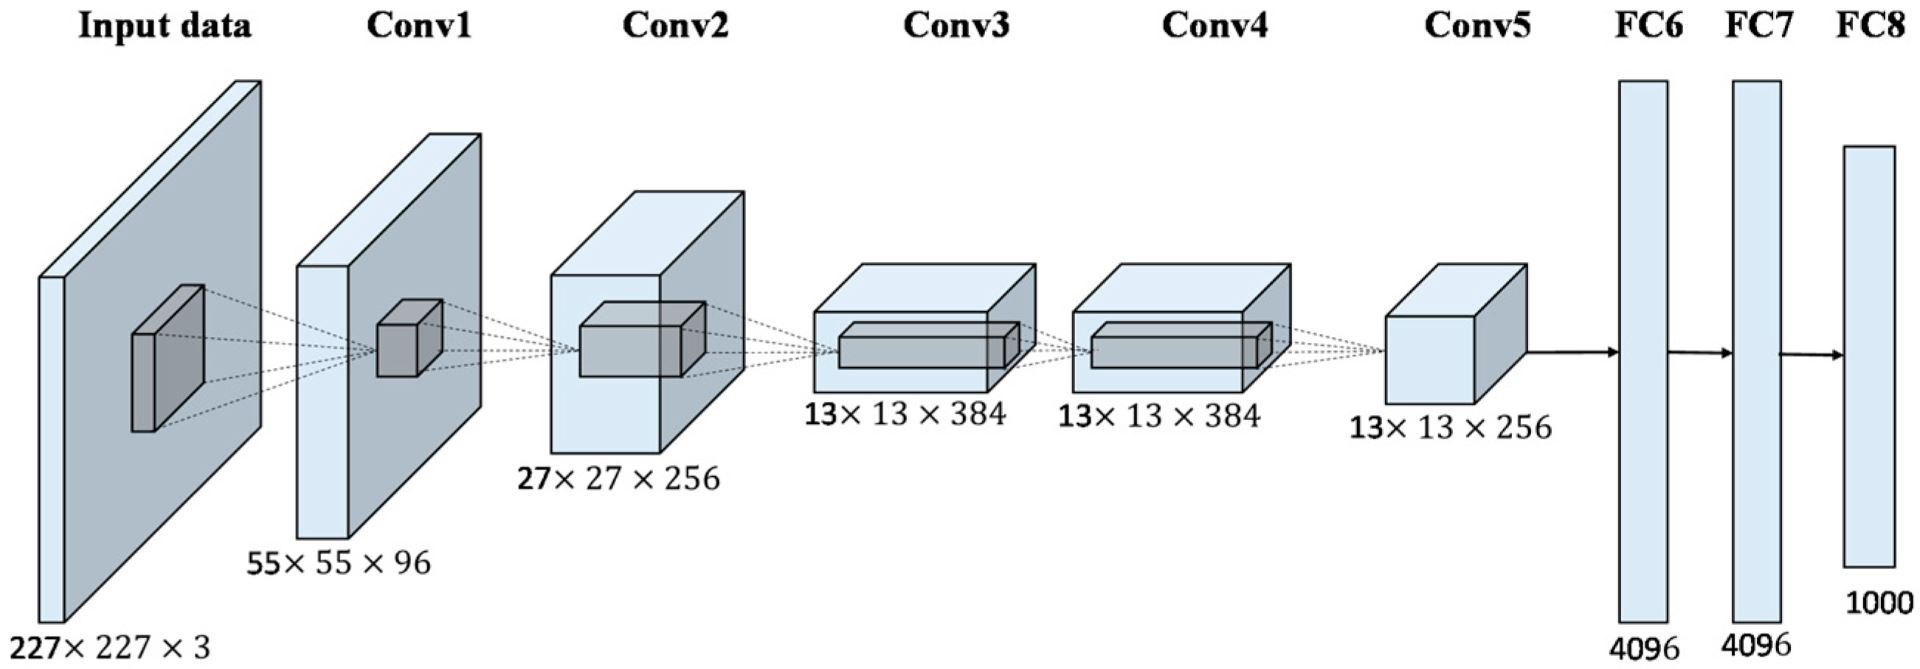
\includegraphics[width=\textwidth]{cnn3.jpg}
\caption{AlexNet - the first work that popularized the use of CNNs and GPUs to accelerate deep learning.}\cite{alexnet, alexnetimg}
\end{figure}
\section{Semantic Segmentation}
\printbibliography[title={References}]
\end{document}
